\documentclass[emulatestandardclasses]{scrartcl}
\usepackage{graphicx}
\usepackage{color}
\usepackage[ngerman]{babel}
\usepackage{hyperref}
\usepackage{fullpage}
\usepackage{calc} 
\usepackage{enumitem}
\usepackage{titlesec}
\newcommand{\todo}[1]{\textcolor{red}{TODO: #1}\PackageWarning{TODO:}{#1!}}
\date{\vspace{-3ex}}
\begin{document}

\title{
	\includegraphics*[width=0.75\textwidth]{ErstesSem/images/hu_logo.png}\\
	\vspace{24pt}
	Hegels Theorie der Weltgeschichte}
\subtitle{Proseminar SS 18\\
          Dr. Dimitris Karydas\\
          Theologische Fakult"at \\ 
          Humboldt Universit"at zu Berlin}
\author{Lennard Wolf\\
        \small{\href{mailto:lennard.wolf@student.hu-berlin.de}{lennard.wolf@student.hu-berlin.de}}}
\maketitle
\begin{abstract}

Hegels Konzept von Weltgeschichte als Fortschritt im Bewusstsein der Freiheit wird im Zusammenhang des Systems des Geistes erläutert. Dem liegt ein Begriff der Geschichtlichkeit zugrunde, der so originär wie bis heute umstritten ist. Die zentralen damit verbundenen Konzepte und Motive von der Vernunft in der Geschichte, der Verwirklichung der Freiheit oder vom Ende der Geschichte werden im Mittelpunkt der Diskussion stehen. Die für Hegels Auffassung von Geschichte ausschlaggebenden Passagen aus den Vorlesungen über die Philosophie der Weltgeschichte, der Enzyklopädie und der Rechtsphilosophie werden gelesen, die auf moodle bereitgestellt werden.
\end{abstract}
\newpage

\tableofcontents
\listoffigures
\newpage


\section{Subjektiver und Objektiver Geist\\(24.04.18)}

\subsection{Organisatorisches}

\begin{itemize}
  \item Moodle-PW: historie (ab 27.04.) geist, manuskripte 
  \item Abgabe: Essay/Protokolle zu insgesamt 10 Seiten
  \item F"ur schein der Teilnahme ist ein Referat/ Protokoll abzugeben
  \item Vortrag am 08.05. Enz. 545 - 552
\end{itemize}

\subsection{Einf"uhrung}

\begin{itemize}
  \item Geist ist geschichtlich
  \item was wir sind wsind wir geschichtlich geworden
  \item Der Löwe versteht sich als Löwe (indem er sich als Löwe verhält ("`an sich"'), nicht reflektierend ("`für sich"')), ohne Bewusstsein zu haben
  \item Metareflektion darüber, wie der Mensch sich auf die Natur beziehen kann
  \item Reduplikation der Weltgeschichte anhand des Begriffs
  \item Subjektivität ist zweierlei: das Wesen des Subjekts (vom Subjekt ist erst in der Moderne zu reden; Das Bewusstsein dass alle \emph{rechtlich} frei sind etc. ist ein modernes) und Reflektion
  \item Die Tiere verhalten sich gesellschaftlich, nur sie reflektieren nicht darüber (Karydas: Hegel ist mit Darwin )
  \item Die Natur hat keine \emph{Geschichte} (was nicht heißt, dass sie keine Historie hat)
  \item Unterschied Historie Geschichte: Wird noch besprochen
  \item Feuerbachs Kernbegriff ist die "`Gattung"'
  \item Empfehlung: Tierphilosophie Hegels
  \item Die Idee: Der Algorithmus der Welt, was die Welt z
  \item Begriffe wie "`Idee"', "`Absolutes"' etc. wurden leider früher immer fetischisiert, doch sie sind auf die Welt zurückzuholen, sie sind ganz naiv, konkret gemeint
  \item die Bewegung vom Abstrakten zum Konkreten ist nach oben gerichtet (erste Negation?)
  \item es spielt das partikulare des Konkreten für das Allgemeine keine Rolle
  \item Der Geist ist das sich von Sich-von-sich-selbst-unterscheiden
  \item Bedürfnis zur Philosophie kommt aus dem Bedürfnis zu Begreifen
  \item der konkrete Geist ist die abstrakte Natur
  \item Der Sohn ist die Natur, die Idee ist der alte Mann
  \item  481: Meint gezeigt zu haben, dass der subjektive Geist ist durch die Form des Allgemeinen vermittelt
\end{itemize}



\section{Objektiver Geist II\\(08.05.18)}

\subsection{Erinnerung}

\begin{itemize}
  \item Übergang von Natur zu Geist
  \item Erst wenn er mit der Anthropologie fertig ist, 
  \item Seele ist noch ein tierischer Aspekt, weil die Reflexion auf sich noch fehlt (unmittelbares Verhältnis) - Eigene Aufhebung
  \item Psychologie hin zur abstrakten Gestalt des Absoluten, alles als Produkt des eigenen Tuns betrachtet wird (Bewegung zum Objektiven Geist)
  \item Philosophie des Rechts muss geklärt werden, um Geschichte verstehen zu können
  \item Das Buch zur Rechtsphilosophie ist eine Polemik gegen die deutsche Rechtsschule
  \item Verhältnis Der Zufalls zur Notwenidigkeit
  \item Das Absolute braucht einen Staat, weil ohne Staat kein Recht und ohne Recht kein objektiver Geist
  \item Es gibt kein Glück in der realen Welt
  \item Wer sich im Staat befindet der ist frei, egal welche Rechtsform besteht
  \item Wo es Zufall gibt, gibt es keine Allgemeinheit (!)
\end{itemize}

\subsection{Anmerkungen zum Übergang vom obj. zum abs.}

\begin{itemize}
  \item Volksgeist (Jena-Hegel): spielt später keine systematische Rolle - was war gemeint, ein Selbstverständnis, das geschichtlich, klimatisch geworden ist
  \item Dialektische Konstruktion muss nachvollzogen werden
  \item Kants ewiger Frieden als Gegenkonstruktion, von der sich Hegel abwendet - wäre unmöglich, da es eine abstrakte negation des krieges wär, wofür keine partikularinteressen für die staaten mehr existieren dürften
  \item Friedensverträge unterscheiden sich vom Naturrecht, vielmehr: konraktualistische Vorstellung vom Recht
  \item Das Recht ist kein Resultat eines Vertrags
  \item Friedensverträge sind die spekulative Bewegung aus Frieden und Krieg - es folgt, dass sie daher aber kein Recht sind
  \item "`Andere Länder andere Sitten"' - Hegel
  \item Wenn der Staat keine klaren Grenzen hat, werden die Menschen versklavt
  \item Marx Argument gegen Kapitalismus ist: Der Kapitalismus kann seine Grundfesten, Land und Kapital, nicht reproduzieren. Er kann nicht in ein Ganzes übergehen
  \item Philosophie kann nur im Tempel passieren
  \item 3 Arten der Geschichtsschreibung in den
  \item Weltgeschichte hier ist die objektive Geschichte und darin gehen die Rectsverhältnisse auf, und alle anderen Verhätnisse aus (Familie, Ökonomie)
  \item Der Staat ist eine Realgestalt des Absoluten
  \item Zur Weltgeschichte gehört beides: Die subjektiven Ereignisse sowie die partialgeschichten des Absoluten 
  \item Der Volksgeist kommt im Absoluten zur Geltung (Kunst, Religion etc.)
  \item Hegel et al haben die Französische Revolution auf den Begriff gebracht
  \item Nächstes mal: §§ zur bestimmung des objektiven geistes 481 bis 468
\end{itemize}


\section{Eigene Notizen}

\begin{itemize}
  \item Subjektiver Geist: Der Mensch als geistige Struktur (Psychologie (Kants Vermögen), Phänomenologie)
  \item Objektiver Geist: Menschliches Miteinander
  \item Absoluter Geist: Wissen des Göttlichen
  \item Bei Hegel ist Sittlichkeit bestimmt als "`Reihe von Pflichten, die wir haben, und die besagt, daß eine auf der Idee gegründete Gesellschaft gefördert und erhalten werden muß"'
  \item Der Staat ist dadurch ausgezeichnet, dass er als Ganzes alle Momente des menschlichen Lebens beinhaltet (familiäres, ökonomisches, politische Institutionen) und sich in seiner Entwicklung auf sich selbst bezieht (ebd.: 330, § 536). Der Staat ist dabei die höchste Weise der Vermittlung von Individualität und Gesellschaftlichkeit, und begründet, beinhaltet und umfasst die familiären und die ökonomischen Beziehungen der Menschen. 
  \item Vernunft ist schon immer da, sie muss nur immer weiter verwirklicht werden
  \item Zirkelschluss? "Daß in den Begebenheiten der Völker ein letzter Zweck das Herrschende, daß Vernunft in der Weltgeschichte ist, – nicht die Vernunft eines besonderen Subjekts, sondern die göttliche, absolute Vernunft, – ist eine Wahrheit, die wir voraussetzen; ihr Beweis ist die Abhandlung der Weltgeschichte selbst: sie ist das Bild und die Tat der Vernunft."'
  \item Ist das Baby dann am Anfang noch Natur
  \item Woher weiß ich dass mein Staat gegen die Befreiung des Geistes arbeitet
\end{itemize}



\section{Objektiver Geist II\\(22.05.18)}


\begin{itemize}
  \item Die Vernunft in der Geschichte
  \item Hat nie die begriffene Geschichte vorgetragen - ist dies überhaupt möglich
  \item Gewaltenteilung ist notwenidge Bedingung dafür, dass alle gleich vor dem Gesetz sind
  \item muss man dann sehen
  \item PR: 273; § 341
  \item von Schiller "`Resignation"': Weltgeschichte ist das Gericht
  \item Das Recht des Weltgeistes/allgemeinen Geistes: die vernünftigen Strukturen
  \item Schwierige Frage ist nach der Notwendigkeit und Zufälligkeit
  \item Vorwurf an ihn: Dass in seiner Geschitsauffassung alles gerechtfertigt war
  \item GW manuskript Band 18 S. 121-129, 1822/28
\end{itemize}

\section{Philosophie der Weltgeschichte - Einleitung 1822-28, S. 121-129\\(29.05.18)}

\subsection{Lektürenotizen}

\begin{itemize}
  \item Dreierlei Weisen des Geschichtsschreibens:
  \item Ursprüngliche Geschichte: seiendes in geistiges umwandeln: Erlebnisse festhalten. Bildung der Geschichte und Bildung des Autors sind das selbe
  \item Geschichtsschreibung braucht einen hohen Bildungsgrad im Volksgeist - und dass sie Geistlichkeit nicht isoliert, sondern im Akt des Geschichtemachens mit vorhanden sind
  \item Reflektierte Geschichte
\end{itemize}

\begin{itemize}
  \item Die Vernunft in der Geschichte ist der Versuch aus den Manuskripten und Mitschriften einen Gesamttext zu erstellen
  \item in der Weltgeschichte, nicht nur die Geschichte von Staaten (Partialgeschichten), sondern die Gestalten des Absoluten, die objektiviert werden, sie haben eine Positivität (Religion, Kunst, Philosophie)
  \item Partialgeschichten kommen mit rein, und es gibt einen Zusammenhang zwischen den Partialgeschichten (und auch untereinander) und dem Absoluten
  \item Wäre aber diese Verbindung herstellbar (ist es theoretisch tragbar und ist es ausführbar?) - die Welt nur als eine Totalität zu betrachten ist schwierig (Marx: die Welt kann ihre eigenen Grundlagen, die zufällig sind, nicht reproduzieren)
  \item Welt als Totalität müsste sich selbst hervorbringen - kein äußeres das einfluss hätte! | da aber Zufälle die Geschichte 
  \item Gott ist sein tun - Bei Hegel gibt es \emph{keine} Negative Theologie: deus absconditus (prinzipiellen Unerkennbarkeit Gottes) - Religion und Philosophie haben einen identischen Inhalt (Vernunft muss auch aus der Religion herausgefiltert werden)
  \item Der Begriff von Anaxagoras: Erstes Dokument der Philosophie (sagt dass der Lauf der Dinge zwar zeitlich ist, aber trotzdem vernünftig ist - vorsokratische Naturphilosophie (Heidegger hat hierzu einen Aufsatz geschrieben))
  \item Die Idealität der Vernunft muss auch Faktizität haben - so wie bei jeder Idee
  \item Als Ordnung der Vernunft ist die Dialektik strukturell begründet
  \item Nur die PHil. verfügt über das Wissen von vernünftigen Strukturen - das ist gerade ihr Geschäft (alles in Schlußform zu bringen (nicht Urteil) - Zufälligkeit ist notwendig)
  \item Wer die Welt vernünftig betrachtet, den betrachtet die Welt auch vernünftig (Rechtsphilosophie)
  \item Referat:
  \item Das was Weltgeschichte ist, dafür reicht unser Alltagsverständnis
  \item aber Philosophie der Weltgeschichte: Weltgeschichte denkend zu betrachten
  \item Es ist unmöglich die Geschichte so zu betrachten wie sie ist - daher ist Betrachtung mit der Vernunft legitimiert!
  \item Nur die Phil. kann den Gedanken der Vernunft benutzen | keine subjektive Idee oder Ideal, nicht bloß so unmächtig, um es nur bis zum Ideal zu bringen, nur als etwas besonderes in den Köpfen zu bleiben | und zwar als Ordnung der Geschichte
  \item Wer in die Sonne schaut wird blind (man steht vor der Abstraktion, und diese macht durch ihre Nivellierung blind vor den Partikularitäten)
  \item Mnemosyne: Göttin der Erinnerung
\end{itemize}

\begin{itemize}
  \item Antigone? dichthonische Ordnung (das Blutbad) vs. ... Ordnung (Recht)
  \item 
\end{itemize}



\section{Philosophie der Weltgeschichte - Einleitung 1822-28, S. 130-137\\(12.06.18)}

\subsection{Sitzung}

\begin{itemize}
  \item Tempel der Mnemosyne: \emph{historia rerum gestarum} | Aufbewahrung dessen, was passiert ist (basale Aufhebung) - 1. Stufe der Verarbeitung - Verschiedene Stufen der Verarbeitung und Ordnung - das ist noch keine Philosophie
  \item Reflektierte Ordnung des Erfahrenen
  \item Begriffene Geschichte: Momente der Realisierung des Geistes aufzeigen
  \item Nicht: Struktur der Logik in Geschichte/Realphilosophie zu suchen (projezieren)
  \item PdG: Tilgung der Zeit: das Denken ist dazu gekommen, nahdem es alle resultate der arbeit der weltgeschicht, verarbeitet hat, redupliziert hat - soll heißen nicht die WG als geschichte der menschheit, sondern der geistdas denken  kommt dazu sich selbst zu thematisieren und seine eigenen regeln herauszuarbeiten (das diamantennetz der verknüpfungen) Vernunft und Logik fallen mit der Geschichte zusammen (Geschichtlichkeit ist nicht zeitlich parametrisiert) - Geschichte hat bei Hegel nichts mit Zeit zu tun - natürlich erscheint sie in der Zeit, sie ist nicht bloßes Sein - aber die Zeit ist eben nur die Form, in der diese Strukturen sich materialisieren - das geistige Prinzip aber ist nicht zeitlich
  \item das Geistige und das Selbstbezügliche
  \item Die Darstellung der Weltgeschichte fängt mit den Indern an (Indien und China: stehen an der Schwelle, haben zwar schon Staatlichkeit, aber bei den Griechen wird die Schwelle überschritten - welche Schwelle? Des selbstbezüglichen?)
  \item Die Zeit ist der daseiende Begriff (der Begriff ist ja ein Vollzug und daher in der Zeit - die Prinzipien sind außerhalb der Zeit) - Das Begreifen kann nur in der Zeit sich vollziehen
  \item Philosophie ist immer post festum (eule) - alle Ergebnisse liegen vor
  \item Notwendig ist der Zufall - die schwierige Dialektik | die Form, die sich objektiviert hat, ist vollkommen kontingent, das Prinzip in ihr ist aber notwendig - das Prinzip scheint erst am Ende durch (!!)
  \item Unterscheidung innerer und äußerer Psychologie
  \item Die Weltgeschichte mag sich von hinten aufrollen (Rückfall in die Barbarei etc.), das Bewusstsein der Freiheit geht aber nicht aus der Welt
  \item Religionsphilosophie ist sehr aufschlussreich für sein ganzes Denken
  \item 4 Partialgeschichten des Absoluten: von Staaten, von der Kunst, der Religion, und der Philosophie - damit wird die Schwelle der Weltgeschichte überschritten (den Begriff der Geschichte macht er an den Griechen fest)
  \item Geist der Zeit muss herausgehoben werden - aber das ist noch interpretation, kein Philosophie
  \item Interessensgeschichte: mit welcher Intention: große (), historische, detailliert
  \item Ein Verzicht auf die Detailumstände
  \item Notwendige Stufenfolge der \emph{historia rerum gestarum}: Livius - lässt Figuren im Geiste der Zeit des Geschichtsschreibers auferleben (Galerie der großen Figuren) - erste naive, dürftige Form der Verarbeitung (versucht auch etwas hineinzuprojezieren)2. Walter Scott, fiktional, wird aus Sicht der Individuen erzählt | (Walter Scott erste Stufe? Nein) | Versucht innere Notwendigkeit aufzuzeigen (an der Schwelle zur Wissenschaft)
  \item “Hegel seems to me to be always wanting to say that things which look different are really the same. Whereas my interest is in showing that things which look the same are really different.” (Recollections of Wittgenstein)
  \item Nächster Schritt: philosophische Geschichtsschreibung
  \item Lynn 1994, the Chinese sages created culture from the hexagrams! -> Creativity in Hegels thought? Hegelianism as foundation to design/gestalten
  \item Is the Glasperlenspiel creative/producing anything? Could Glasperlenspieler design something new?
  \item Hegel benötigt die sinnlose these, dass das absolute Bewusstsein der Freiheit ewig im Allgemeinen ist, wenn es nur einmal partikular bestand, da ansonsten seine begriffene Geschichte nicht wahr sein kann. Seine begriffene Geschicte kann aber nicht wahr sein, daher braucgt es diese annahme nicht
  \item Hegel nicht hegelianischer machen als er ist!!! Das hätte man ihm sagen müssen
  \item 
\end{itemize}

Gedanken

\begin{itemize}
  \item 
\end{itemize}




\section{Philosophie der Weltgeschichte - Einleitung 1822-28, S. 130-137\\(12.06.18)}


\begin{itemize}
  \item Ab Seite 150:
  \item Orientalen nur einen Menschen als frei
  \item Mittel 
  \item Der Endzweck der Weltgeschichte ist, dass der Geist an und für sich frei ist
  \item Es sind die Individuen, die Weltgeschichte hervorgebracht
  \item Schlachtbank, auf dem das Schicksal der Völker: Wem sind die
  \item Ab 157 gehts richtig los
  \item Frage nach Beziehung von Innerliches und Äußerliches (was?)
  \item Es brauch das partikularinteresse
  \item Zweite wesentliche Moment der Freiheit: dass die eigenen interessen (und die Möglichkeit dies zu tun) verwirklicht zu werden gewollt wird ("`das absolute Recht des SUbjekts"') - Individuum hat Rechtsanspruch auf 
  \item Bei Hegel ist Freiheit auch positiv bestimmt! Das heißt du bist berechtigt, zum Beispiel deine eigenen Interessen durchzusetzen. Negative Freiheit gibt es natürlich auch
  \item Hegel nivelliert das Individuum nicht für die Gemeinschaft!
  \item Verbrechen: Verstoß gegen die Rechte eines anderen, aber auch ein Verbrechen gegen die Allgemeinheit! Es folgt, dass das Verbrechen sich gegen einen selbst richtet. Wie kann man das rechtfertigen? Alle Individuen sind mit der Allgemeinheit vermittelt, 
  \item Man ist frei "`insofern"', nicht einfach so
  \item Englisches Recht hatte Hegel probleme mit (wegen )
  \item Große Figuren sind nicht nur Katalysatoren, sondern \emph{Werkzeuge}
  \item 166 bis 167: Sehr wichtig und eindeutige Stelle!! Individuen sind Werkzeuge des Weltgeistes aber auch Selbstzweck (wird an Sittlichkeit und Religiosität festgemacht, wegen allgemeinen Inhalt, dem praktischem Verhältnis zur Welt, Religiosität als theoretischem Verhältnis zu Welt)
  \item Für den Weltgeist an der Zeit: Was objektiv möglich ist! Es war vorher nicht möglich - Das mögliche wird nur nach der Dämmerung erkannt
  \item Kritik wäre: Es gibt nicht den einen Weltgeist! 
  \item Verhältnis Zweck und Mittel?
  \item Individuen haben Teil am Vernunftzweck, Freiheit steht darin, gutes und Böses zu wollen und können dadurch schuld haben
  \item 168 (!!) : Was die menschen moralisch unzufrieden macht, besonders heutzutage ...
  \item 2 Denkfiguren: Kritik des Sollens (Kritik des Sollens im allgemeinen oder in der Philosophie?) - Problematik der schönen Seele: Enttäuschung über Entwicklungen des Zeitalters, die man zu überwinden sich versprochen hat, und wird dadurch an/von der Welt gekränkt
  \item Kritik des Sollens: 168f
  \item Kritik an Stoa: "`Welt ist böse, kann man nichts machen"'
  \item Zeitdiagnose: Alle gehen im Namen des Rechts! Wie ist das zu handhaben? 169 (Niemand sagt dass er gegen die vernunft arbeite)
  \item Uhr nur mit jetzt
  \item Immer eine Distanz zwischen Prinzip und individueller Umsetzung; weil Individualität immer Grenzen hat (Philosophie)
  \item Die in der Realität umgesetzte Freiheit ist immer eine Defiziente
  \item Inhalt ist die Bewegung der Form; 
  \item Vernunft muss immer Eingesetzt werden
  \item Freiheit ist immer ein Spannungsverhältnis zwischen Prinzip und Realität
  \item Hätte rechtsgeschichte schreiben müssen
  \item Religionsgeschichte und Philosophiegeschichte?
  \item Von Geist zu sprechen geht erst wenn man schon Wissen von sich hat! Deswegen muss Staat schon vorausgesetzt werden!!! Standpunkt der konkreten Allgemeinheit!!!
  \item Kein Apologet des Staats, aber Apologet des Rechts!
  \item "`Schlechtes Sollen"' 
  \item Abstrakte Veränderung überhaupt: enthält den Fortgang zum Besseren
\end{itemize}


\section{Philosophie der Weltgeschichte - Zweckmittelrelation\\(12.06.18)}

\subsection{Protokoll zum letzten mal}

\begin{itemize}
  \item Schlüssel dafür, dass es irgendwie in der Geschichte Vernünftig zugeht
  \item das muss man erstmal schlucken aber auch verstehen (alles nur Kontext dessen, dass dieses Konzept zur Angriffsfläche gegen Hegel - von der krassen Missdeutung, alles und auch Hitler wäre vernünftig, mal abgesehen)
  \item Erzählt von Frau: Dissertation, mit Preisen, aber alles falsch gedeutet - aus Mitleid mit den Opfern
  \item Was macht die Weltgeschichtlichen Figures zu solchen? (Caesar, Napoleon etc. warum nicht mehr beispiele? weil ist egal) anhand der Zweck Mittel Relation erklärt? Was haben sie vermocht? Dass das was an der Zeit war zusammen fällt mit ihrem subjektiven Willen (Individuen kkönnen nur ihre e) Kein Individuum kann Einblick in das dezietige Weltgeschehen haben!
  \item Es hat sich ergeben, dass der Wille dieser Individuen das zum Ausdruck gebracht hat, in welcher auch immer defiziente, pervärtirter Weise umgesetzt hat, was an der Zeit ist (was objektiv möglich ist, dass unendlich komplizierte Geflecht der objektiven Bedingungen reif waren/sich so stellten, dass dieser Wille etwas bestimmtes im Rahmen der obj Bedingungen (äußerliches Staatsverhältnis) vorantreiben) - das stellt unentbehrlichen ANhaltspunkt
  \item die Verhältnisse werden real Richtung Freiheit umgestaltet 
  \item Weltgeschichte ist der Fortschritt
  \item Unterscheidung geistige Geschichte und materiale Geschichte??
  \item Programm: Hegel will die theoretischen Thesen mithilfe der Zweckmittelrelations sättigen
  \item Differenzieren: Wille lässt sich nie realisieren wie man es im Kopf hat (gerade weil man sich anpasst (mittel zum zweck und umgekehrt)) - Marx: die menschen machen die Geschichte nur hinterrücks (sie wollen was erreichen aber das was sie erreichen kann nie so aussehen wie sie es konzipiert haben - klar)
  \item Napoleon ist so wichtig wegen des Code Napoleon: "`alle sind frei"'
\end{itemize}


\subsection{}

\begin{itemize}
  \item Fortgang zum Besseren ist Fortgang vom Bewusstsein zur Realität
  \item In der Natur passiert nichts neues
  \item Evolution ist nicht als Geschichte zu verstehen! Geschichte ist Geist. Evolution ist nichts neues (Was bedeutet das Neue bei Hegel? Oktoberrevolution ist was neues, weil die Freiheitsverhältnisse sich verändert haben; Hitler nicht, Hitler hätte man verhindern können)
  \item Hitler ist für Hegel nicht Geschichte - das hat nichts mit Freiheitsverhältnissen mehr zu tun ausser dass sie eingeschränkt wird wieder!!
  \item Wann ist \emph{post festum}? 
  \item Pointe: \emph{Trieb der Perfectibilität} - nicht bloß Gedanke des Fortschrittsglaubens
  \item Geschichte ist Bewusstsein, das die Welt wieder redupliziert als vernünftie Struktur
  \item Kants Weltbegriff der Philosophie?? wasdas?
  \item Perfectibilität bleibt erstmal abstrakt! Das Ziel ist unbestimmt! Der Mensch vervollkommnet sich - bloß eine abstrakte moralische Vorstellung. Man kann nicht von dem Menschen sprechen, sondern nur von individuen in bestimmten historischen Verhältnissen
  \item Was meint er wirklich mit Entwicklung? Unterschied Entwicklung in Natur und im Geist: Natur immer eingeschränkt, keine wirkliche Veränderung (egal wie viele Papageiarten)- Geist wirkliche veränderung
  \item nAtur ist ist äußerlichkeit der veränderung - die Erinnerung der Natur bleibt - der Geist ist der Prozess der Abstreifung der Natur
  \item Unterschied Tier zu Mensch: nicht sooo stark: In der Natur gibt es keine Taten, beim Menschen schon! (Mitte des subjektiven Geistes)
  \item Entfremdung hier: Schon in der PdG: Wesentlichen Moment des Geistesbegriffes überhaupt: genau wie in dem Sinn auf S. 184 - Schon bei Linkshegelianern (kritische Wendung als wichtige Interpretation): Grundlegende Kategorie des Sozialen (Honneth), sowie öffentliche Diskussion; Feuerbach, junger Marx; Debatte bei 60ern: Interpretation des Begriffs der Entfremdung, indem das bleibende Moment ignoriert wird und sich mit dem kritischen nur auseinandergesetzt wird (Gattung?) | Für Hegel aber ist Entfremdung zentrales Moment des Geistes: der geist wird sich fremd, insofern als \emph{dass er etwas produziert} (dadurch ist die römische Gesellschaft zerfallen (?))
  \item Entwicklung des Geistes ist auch Hervorbringen eines Zwecks!
  \item Selbstzweck, Selbstbezug, Selbstbewusstsein, Freiheit (bei sich sein im andern)
  \item Lacan: Spiegel bei Kindern wo erkennt sich das kind das erste mal? im Spiegel: "`Das Spiegelstadium"' (Aufsatz)
  \item Eugen Fink: Über die Phänomenologie des Geistes
  \item Weltgeschichte stellt die Entwicklung des Prinzips als Stuffengang dar (im Bezug auf die Freiheit)
  \item Stuffen wegen geistigen Schritten!
  \item Das Resultat um das geht es - Geist ist auch resultat, von wem? von sich selbst!
  \item Das ist die Pointe, agiert nicht selbst, sondern mit den Menschen, mit ihren problematischen einzelwillen
  \item Dass er sich selbst als das Resultat erkennt
  \item Text zu ende diskutieren - dann och 3 sitzungen - dann vorschlag was wir noch lesen (Mitschriften/Religionsphilosophie)
  \item Hayden White - theoretiker der geschichtswissenschaft - Geschichte kann nur erzählung sein (gegenentwurf zu Hegel)
\end{itemize}


\section{Der Stufengang, S. 130-137\\(03.07.18)}

\subsection{Protokoll zum letzten mal}


\begin{itemize}
  \item Geschichte stellt sich so ein, dass das was die mannigfaltigkeit von partikularinteressen am ende eine vernünftige struktur hervorbringen
  \item was macht eine vernünftige struktur aus?
  \item resultat ist der geist insofern, als dass zum geist das wissen von sich gehört
  \item wissen (nicht im schulischen sinne) die wirklichkeit ist ein produkt von ihm; Recht gehört auch dazu
  \item Endziel: Monarchie
  \item Veränderung/Entwicklung
  \item Was ist das wirklich Neue in der Geschichte was die Natur nicht hervorbringen kann
  \item Inwiefern ist Darwinismus damit kompatibel?
  \item Evolutionstheorie: Aus der Geologie - wie kommen fossilien auf den berg?
  \item Erste Idee: Erde hat sich verändert
  \item Logisches Fassen des Unetrschiede zwischen Natur und Geist
  \item Er ist kein Schöpfungstheologe - es ist so wie es ist und dazu kann Hegel nichts sagen (Erschließt die Schöpfung begrifflich aus)
  \item Aufklärung als "`Naturgeschichte der Vernunft"' wie kann Aufklärung in Dogma umschlagen (PdG - Dialektik der Aufklärung bei Hegel?) - Adorno Horkheimer anderes verständnis von Vernunft (SPaltung des Vernunftbegriffs: positiver und negativer - )
  \item Adornos Definition von Fortschritt: Von der Steinschleuder zur Atombombe
  \item Vernunft als den Grund (Substanz) von Freiheit
  \item Dilthey: Historische Vernunft
  \item Im Reiche des Geistes löst eine Figur des Geistes die vorige ab, z. B. folgt der Gotik die Renaissance. Die Grenze setzt der neue Stil, der einen Bruch im alten Stil darstellt. Hegel nennt diese Brüche auch \emph{qualitative Sprünge}. In der Natur gibt es für Hegel allerdings keine solchen Sprünge; sie kehrt nur ewig in sich selbst zurück.
  \item zeitlich ist die Natur vorranging, aber logisch ist der geist vorrangig
  \item In der absoluten Idee ist die Natur abgeschweift
  \item Tragödie hat gezeigt dass der Geist sich bewusst ist
  \item Marx: Prometheus (Naturbeherrschung) // Hegel: Herakles, weil er den Menschen die Politik gebracht hat (ansonsten wäre die Menschheit zu sklaverei verdammt) -- Deutung der Mythologie
  \item Derrida: Der Schacht und die Pyramide
  \item Borges: chinesische wissenschaft
\end{itemize}

\begin{itemize}
  \item 3 STufen: einer ist frei, einige sind frei, allgemeine freiheit
  \item Geschichte erst ab dem moment, wo vernünftigkeit weltliche existenz hat
  \item Wo diese Stufen noch nicht angefangen wurden zu betreten ist noch keine geschichte!
  \item Altes Indien: Geschichtschreibung ist als Naturgeschichte zu verstehen
  \item Der begriff ist die Zeit
  \item Art des Ganges
  \item eigentümliches Prinzip ist Geist eines Volkes
  \item Volksbegriff problematisch: 
  \item Geist ist für sich nicht frei - ein subjektiver geist wird frei.....?
  \item Entwicklung des subjektiven geists ist auch nicht 
  \item Unterschied ist der Gehalt
  \item Formalismus: 2 Arten: 
  \item Weltgeschichte bedeutet, wie es sich im Lichte des Prinzips der Freiheit stellt
  \item Das einzig gehaltvolle ist die Freiheit - der Rest ist nur Form
  \item Kein Gehalt in reiner Kategorisierung/Beschreibung (chinesische wissenschaft)
  \item 1. Band Vorlesungen Aus der Philosophie der Religion: Deutung der Mythologie und der antiken Götter um 365 - (mehrere seiten) fängt mit kronos (kosmologie ) an
  \item 
\end{itemize}


\section{Der Stufengang, S. 130-137\\(03.07.18)}

\subsection{Lektürenotizen}

\begin{itemize}
  \item Bestimmung = Bestimmtheit; 
  \item Vollständige Bestimmung vollzieht sich in der Schlußform
  \item vernünftige Bestimmung hätte die Form des Schlusses A B E
  \item Periodiserung muss man ganz doll erstmal können!
  \item 30 40 Paragrafen der Rechtsphilosophie
  \item Anderer Weg: Differenzschrift (früher Jena Hegel - hat aber große differenz in der konzeption des absoluten - aber man kann schon gut unterschied zu kant fichte schellng) 
  \item Bei Phänomen. Die Einleitung eher zum Einstieg
  \item Jaeschke: Handbuch ist die erste Adresse (das wichtige: keine idiosynkratische interpretation)
  \item Die Klassische Deutsche Philosophie nach Kant: Systeme der reinen Vernunft und ihre Kritik 1785-1845
  \item Vittorio Hösle Hegels System eher nicht gut!
  \item Gamm reclam Der Deutsche Idealismus: Eine Einführung in die Philosophie von Fichte, Hegel und Schelling 
  \item christian eber suhrkamp (vorlesungen in prag)
  \item serie mhrere bände: suhrkamp der weg zum system - hegels praktische philsophe (ok) - enzyclopädie ---- alles eher idiosyncratisch (Christoph Jamme und Helmut Schneider)
  \item flasch: analytische interpretation, die dann wichtiger genommen wird als der text selbst
  \item Hegel und Heideger sind die größten philosophiegeschichtler - beide mit eigenem system
  \item steelmanning ist wichtig
  \item einfach erstmal schreiben - der anspruch ist nicht hier die wahrheit zu schreiben
  \item Das System bedingt dass man überall anfangen kann - es kommt auf das gleiche hinaus, denn es sind kreise die sich schließen
  \item immer mit einer referierenden frage: eine interpretation eines bestimmten abschnittes!!!!! 
  \item es wird über allg und einz gesprochen - es wäre verfehlt das neu zu definieren - das wäre ein thema für sich. 
  \item wenn man nicht schreibt hat man da nichts kapiert - wenn es keine form annimmt bleibt es nichtig
  \item Man kommt an thomas mann erst heran wenn man über ihn schreibt - THOMAS MANN
  \item so nehmen die gedanken form an
  \item einen eigenen ansatz zu haben ist etwas anderes (dünner) als eine eigene interpretation zu haben (honneth et al kommen folglich eher dünn daher)
  \item hegel hat kannt auf eine bestimmte art und weise interpretiert - auch wenn man mit kant gegen hegel argumentieren kann: hermenautik oder dialektik oder analytische sprachphilosophie? was ist das richtige verfahren? Es scheint aber an allen was dran zu sein!
  \item Auch nicht bei masterthesen, nicht bei dissertation sollte der anspruch einer eigenen these sein - interpretieren soll man. pointieren, was man daraus verstanden hat!
  \item hegel philosophiert ohne voraussetzungen, auch wenn man trotzdem immer dinge mitdenken muss
\end{itemize}


\begin{itemize}
  \item meiner seiten gleich mit der blauen fassung (band 4 a) Vorlesungen über die Philosophie der Religion | Teil 2: Die bestimmte Religion
  \item Meiner 434: religion der menschlichkeit, wo das göttliche menschlich dargestellt wird
  \item was der mensch konret ist wird als göttliches dargestellt (projketionsurthese)
  \item 3 seiten: Gehaltvolle, gttlichkeit in der wesentlichkeit . fatum . äußerlichen einzelheiten
  \item Was den reinen gehalt betrifft: das ist immer die substantielle grundlage der vernünftigkeit - die wesentliche freiheit
  \item hier: dass der mensch sich als göttliches darstellt (das wird im christentum noch weiter getrieben)
  \item deswegen erklärt er das griechische als das, wo alles anfängt - denn darin bringt sich die freiheit das erste mal zum ausdruck
  \item wesentliche freiheit in ihrer bestimmung, die freiheit ist somit die sittlichkeit, vernün
  \item die freiheti ist das sich bestimmen, das formelle
  \item dass dieses umschlägt in die sittlichkeit, das setzen wir voraus (das ist in der rechtsphilosphie zu klären)
  \item Auseinander: an sich und für sich sind getrennt
  \item dass es naturgötter gibt (ab der stelle geht es los) - aufzählung, kernus die meere, hyperion: sterne, zeichen der dämmerung, chronos: zeit, 
  \item naturgestlatungen sind die titanen - sind auch personifiziert, aber nur oberflächlich - natürliche mächte, keine geistige macht
  \item helios ist nicht der gott der sonne (als von dieser getrennt), das sagen die griechen nicht, die sonne ist der gott selbst!
  \item das geistige hat sich über die titanen erhoben und beherrschen nun die welt - götterkireg! in diesem krieg liegt die ganze grundlage der griechischen myt7hologie, dass sich der geist über die natur ermächtigt haben
  \item mehr tun die götter nicht!
  \item es ist eine erkenntnis der griechen selbst
  \item am anfang war das chaos (klassische codifizierung essyot??), die schwarze nacht
  \item kosmogonie die auch eine theogonie ist, chronos, der vater aller götter, (hängt mit zeit zusammen) er hat seine kinder gefressen, genau so wie die zeit die eigenen momente verschlingt | dem wird aber einhalt geboten: die olympischen götter (die kinder des chronos) hat er nicht mehr verschlingen können, und so wurde er vom thron gestürzt. Chronos wurde nicht getötet (zeit würde still stehen), sondern man nahm sich die gestaltung der zeit an! Auch nicht gedemütigt, haben noch ihre ehre, die naturmächte sind noch vorhanden
  \item Die Dieke (gerechtigkeit), nemesis (formelle?), eumäniden, styx etc, werden zu ihnen gerechnet! - bloß an sich seinende mächte, die auch geistig sind - aber nur in sich seiende geistigkeit nur abstarkte ruhe, abstrakte geitigkeit ist, so sind sie den alten göttern zugerechnet. geistigkeit ist also noch eine innerlich seiende macht, also natürlich!
  \item höchste macht auf erden
  \item prometheus: konnte nur das feuer bringen, aber nicht die sittlichkeit, die politeia! |  wird gefesselt, leber wächst wieder nach etc. 
  \item mit zeus hat staatlichkeit angefangen zu gelten: Gott des Staates
  \item Ödipus: Er war schuldig weil er das getan hat! Also muss er büßen! Moderne konzeption dass er das wissen musste galt nicht - die eumenyden werden nicht aus der stadt verbannt, das wäre fatal! sie werden gebändigt!
  \item IN der moderne: die macht die immer noch da ist, das vehätltnis zwischen moralität und sittlichkeit, das (schlechte) gewissen!
  \item ABstrakte Betrachtungen: Götter sind verstreut, nicht weise, konkrete bestimmungen
  \item das schicksal ist ohne zweck, "`ist so passiert"'
  \item Das abstrakte kann nicht begriffen werden, begreifen heißt etwas in seiner wahrheit wissen
  \item Götter: Von Menschenhänden gemacht (gedichtet nicht erdichtet?), das auseinanderfallen der geistigen Mächte (Priester waren Göttermacher) | das göttliche wird nicht im geiste oder in der wahrheit begriffen (kann sein dass ich mich verhört habe)
  \item Es hat die Form des geistigen, indem es schön ist
  \item Athene besonnders bemerkensert... stelle ist interessant
  \item Übergang zum christentum: ein mensch erhebt sich zum fatum aller anderen
  \item das fatum der griechen war die römerwelt
  \item erster schritt zur freiheit: jüdischer Monotheismus
  \item Wichtiger Zusammenhang hier: Religion und Politik!!!
  \item Gibt es geistige Momente in den Göttern, aber diese coexistieren
  \item Im Polytheismus bleiben die Götter einzeln und damit endlich, die fantasie hat sie hervorgebracht; so kann man die Göttlichkeit am Ende aber nicht denken!
  \item mit der reformation kann man die vorstellung von gott auch denken
  \item Rom: Kaiser wurde zum Gott - daran ist es zerfallen und das waren die Geburtswehen zur Rekigion der Wahrheit
  \item Ägyptische Religion: Anthropomorph aber immer noch naturphilosophie!
  \item Griechische Religion schwelle zur Geschichte!
  \item Jesus ist Gottes- und Menschensohn. Deus .. anthropo
  \item Hegel polemisiert gegen Negative Theologie - Adorno und Horkheimer finden gut!
  \item ZUm nächsten Mal: Alte Meiner: erster band, suhrkamp über das antike griechenland anderer band: 
\end{itemize}


\begin{itemize}
  \item polys: erste (nicht zeitlich) form der staatlichkeit
  \item vermittlung z Allg d freiheit schon da
  \item fängt mit den indern an
  \item gegen die reformbill!! nicht konservativ sondern dialektisch.(?)
  \item schwelle beginnt mit der hölenmalerie (ist kunst und es wird festgehalten) nur das macht ohne eine vernünftig gefasste allgemeinheit kaum sinn, denn der bezug zur allgemeinheit fehlt
  \item rechtsphilosophie ist bei ihm kein sollen! ist nicht der ideale staat! es geht desckiptiv los
  \item in der rechtsphilosophie geht es darum, wie man den staat vernünftig zu fassen hat
  \item teleonomie?
  \item MARX 500 ARTIKEL new york tribune
  \item winkelmann: die ewige ruhige strahlende weiß und blau
  \item "`schlimmer für die tatsachen"' - das äußerliche ist immer kontingent und unwichtig im gegensatz zum prinzip
  \item der zerfall des shintoismus
  \item kann man vern strukturen erkennen, nach denen 
  \item band 18 2. teil religionsphilosphie ende griechische
  \item dann in die vorlesungen reingucken
  \item id_phil@hotmail.de
\end{itemize}





%\section{Ideen zu Hausarbeit}
%
%\begin{itemize}
%  \item Es ist keine Whig history, da nicht gesagt ist, dass der Geist zwangsläufig die Freiheit erlangt, es ist vielmehr einfach eine Sache der Zeit
%  \item Indem der Fokus auf den subjektiven Geist zurückgelenkt wird, die Sittlichkeit als schädigend für den subjektiven Geist aberkannt wird und der objektive Geist zum Werkzeug für die erfüllung des subjektiven Willens umgekehrt wird, befinden wir uns in einem für den Geist regressiven Zeitalter
%  \item Zufall und Notwendigkeit beim Fortschritt, whig, moldbug
%  \item Theodor W. Adorno schrieb in der "Minima Moralia": "Liberalität, die unterschiedslos den Menschen ihr Recht widerfahren lässt, läuft auf Vernichtung hinaus." Und fuhr fort: "Wie der Wille der Majorität, die der Minorität Böses zufügt und so der Demokratie Hohn spricht, nach deren Prinzip sie handelt." 
% Gegen die Reformbill???

%\end{itemize}
%
%
%
%\newpage
%\section{"Uber den Professor}
%Prof. Mustermann ist..


%\begin{figure}[h]
%	\centering
%	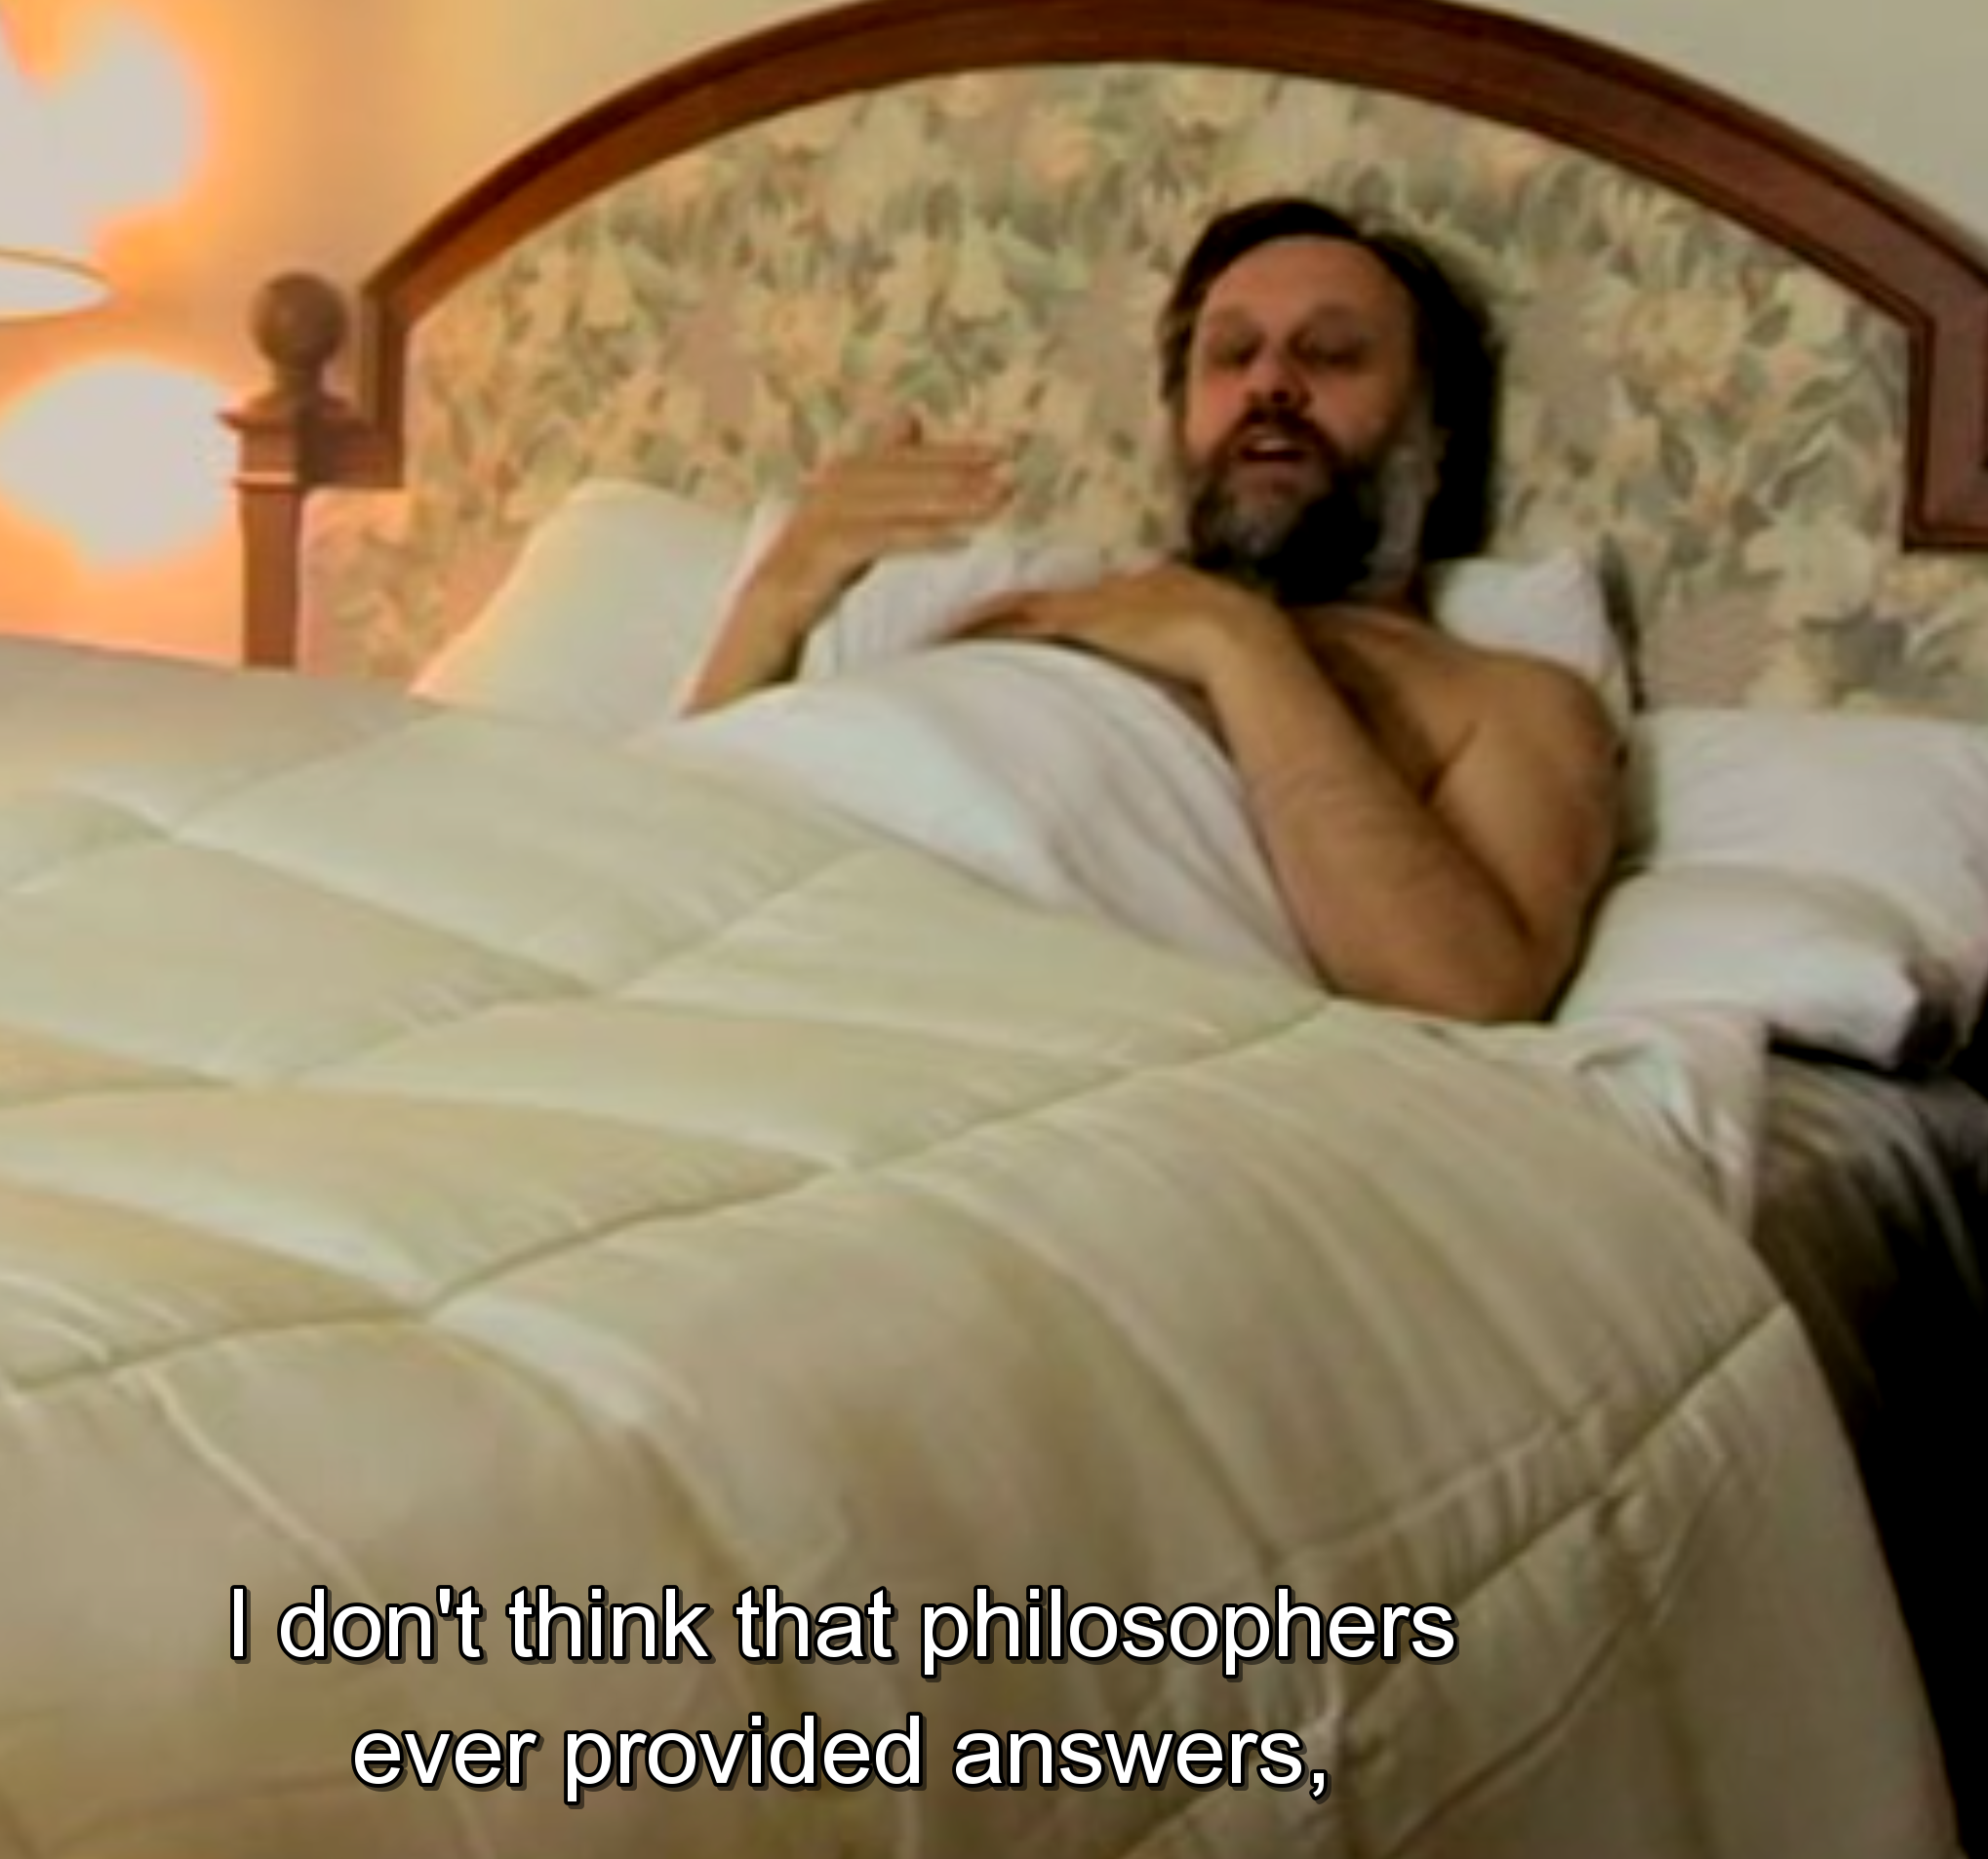
\includegraphics[width=0.5\textwidth]{images/template.png}
%	\caption{Template Bild}
%	\label{fig:template}
%\end{figure}

\end{document}
